\documentclass[10pt,twocolumn,letterpaper]{article}

\usepackage{cvpr}
\usepackage{times}
\usepackage{epsfig}
\usepackage{graphicx}
\usepackage{amsmath}
\usepackage{amssymb}

% Include other packages here, before hyperref.

% If you comment hyperref and then uncomment it, you should delete
% egpaper.aux before re-running latex.  (Or just hit 'q' on the first latex
% run, let it finish, and you should be clear).
\usepackage[pagebackref=true,breaklinks=true,letterpaper=true,colorlinks,bookmarks=false]{hyperref}

% \cvprfinalcopy % *** Uncomment this line for the final submission

\def\cvprPaperID{****} % *** Enter the CVPR Paper ID here
\def\httilde{\mbox{\tt\raisebox{-.5ex}{\symbol{126}}}}

% Pages are numbered in submission mode, and unnumbered in camera-ready
\ifcvprfinal\pagestyle{empty}\fi
\begin{document}

%%%%%%%%% TITLE
\title{UFo - Coupling Uncertain Active Constellation Models with \\
Cascaded Forest Predictors for Sematic Segmentation}

\author{First Author\\
Institution1\\
Institution1 address\\
{\tt\small firstauthor@i1.org}
% For a paper whose authors are all at the same institution,
% omit the following lines up until the closing ``}''.
% Additional authors and addresses can be added with ``\and'',
% just like the second author.
% To save space, use either the email address or home page, not both
\and
Second Author\\
Institution2\\
First line of institution2 address\\
{\tt\small secondauthor@i2.org}
}

\maketitle
%\thispagestyle{empty}

%%%%%%%%% ABSTRACT
\begin{abstract}
We consider the task of model-based semantic segmentation. The model is described by a constellation model of parts that are represented by active shape- and appearance models. We term this an active constellation model. As a running example we utilize a 21-part, chain-based spine model of a zebra fish observed in microscopic images. The prevailing approach to solve this task is to first generate pixel-independent features for each part, e.g.\ via a cascaded decision forest predictor, which are then fed into an MRF-based model-fitting objective to infer the optimal MAP solution of the constellation model. Our key contribution is to abandon this static, two-stage approach and mix feature generation and model-based inference in a new, more flexible, way. In particular we interleave the cascaded forest predictors with inference steps for the model-fitting. A key finding is that “uncertain” model-outputs at intermediate stages of the cascade, in the form of part-based marginals, are essential for best performance. 
%
This is because, as opposed to MAP inference, the soft marginals do not commit to a certain -- potentially wrong -- solution ``at first sight''. If unsure at first sight, soft marginals allow for ``narrowing down'' on the correct solution in later stages of the cascade. 
%
We validate our findings with an in-depth study of alternative inference steps, including popular geodesic smoothing as well as MAP inference. %, and alternative output generation steps, including max-marginals. 
We believe that our findings are not only relevant for other types of constellation models, but, more generally, for the recent trend of combing deep learning models with physically-motivated structured models. 
\end{abstract}

\begin{figure*}[t]
\begin{center}
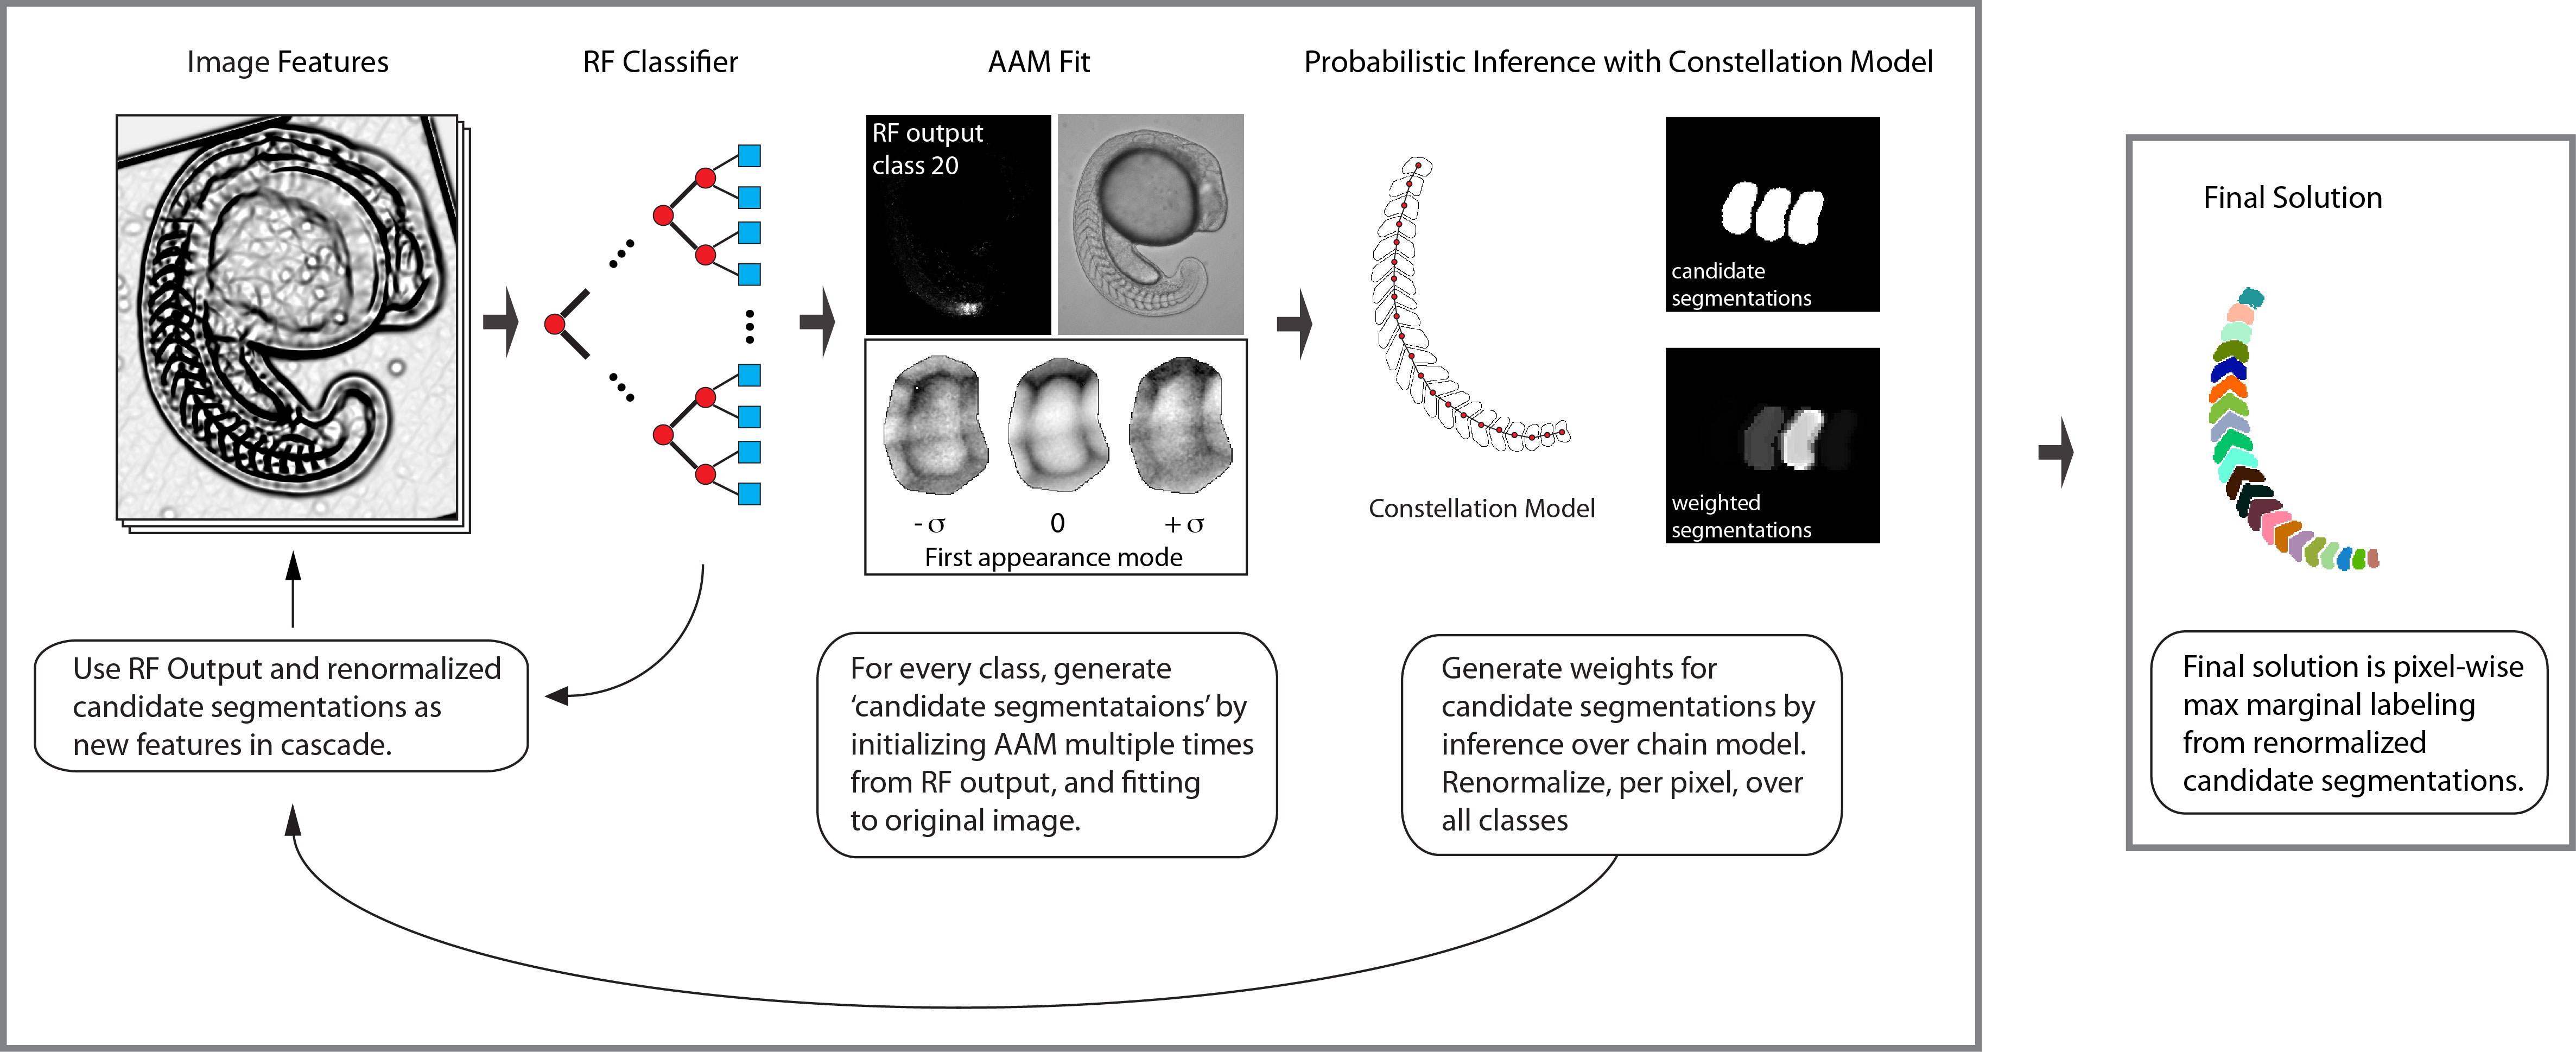
\includegraphics[width=\textwidth]{pipelineBIG.jpg} %&[trim=0cm 2cm 0cm 1cm,height=0.2\textheight]
\caption{Pipeline.}
\label{fig:pipeline}
\end{center}
\end{figure*}


\section{Introduction}
Many tasks in computer vision have as input an image and as output a dense labeling, where each pixel is assigned one out of many pre-defined classes. An example is a sematic segmentation of a person in an image, where each pixel is assigned a label such as “background”, “left leg”, or “head”. 
%
So-called structured models, such as a Conditional Random Field (CRFs), are often used for semantic segmentation. 
Depending on the prior knowledge about the task at hand, the underlying graph may be a (super-)pixel grid, or a graphical constellation model that captures relative locations of multiple parts of an object. 
%
%Furthermore, knowledge about distinct shapes of sought objects or parts of objects is often captured by means of statistical shape and appearance models. 

Such structured models commonly capture the task of semantic segmentation via an objective function that is composed of a data term and a prior. 
%
The data term, referred to as ``features'', is derived from the image at hand, yielding pixel-wise distributions over class labels. The prior is enforced subsequently. 
%
% from image data that gives for each individual pixel a distribution over class labels. These class-label distributions define the unary potentials in the CRF
%
Current state-of-the-art approaches typically employ pixel-wise classifiers combined with MAP inference on a (super-)pixel grid graph for semantic segmentation (e.g.\ \cite{funke2014candidate,}), or on a graphical constellation model for the localization of object parts (e.g.\ \cite{Glocker2012,Glocker2013,TeethMICCAI2012,SeifertAnatomicalSPIE2009}).  
%
A recent trend in computer vision is to learn deep, \emph{cascaded} models for feature generation, such as CNNs~\cite{NIPS2012_4824} (see also e.g.\ \cite{funke2014candidate}) and Auto-Context Models~\cite{AutoContext2008} (see also e.g.\ \cite{PoseMachinesECCV2014}). 
%
These models play the role of learning a complex non-linear mapping from images to features which are relevant for the task at hand. 

This modelling framework is however very static, as it separates feature generation and inference (i.e.\ "`model fitting"'). 
%
It has been shown that better features can be generated by \emph{interleaving} feature generation with MAP inference in pixel-grid structured models~\cite{DTF,RTF,UweCVPR2013} 
%
or model agnostic smoothing smoothing~\cite{GeoForests2013}.\footnote{Note that this is different from the classical "`hierarchical"' approach that, purely for the sake of run-time, performs feature generation and inference multiple times on different scales (see e.g.\ \cite{CootesECCV2012RRFandSSM,CootesFemurTMI2013} [check!]).}

In this work we take the idea of interleaving feature generation and inference a step further: 
%
Instead of interleaving feature generation with a pixel-level structured model or model-agnostic smoothing, we interleave with a global, generative \emph{active constellation model}. By this term we refer to a graphical constellation model, where the individual object parts are captured by \emph{active appearance models}~\cite{CootesAAM2001}. 
%
We suggest a cascaded pipeline, as illustrated in Figure~\ref{fig:pipeline}. 
% 
The most important aspect of this cascade is the question of what to infer from the constellation model at intermediate stages of the cascade. 
%
Options are marginal distributions or the MAP solution. A model-agnostic, yet ``image-aware'' alternative to model-based inference is geodesic smoothing~\cite{GeoForests2013}. 
%
One of the main aspects of this work is to study the trade-offs that come with these options. 

We show that marginal distributions are a clear winner for an exemplary application of semantic segmentation of many self-similar structures, namely vertebrae in spines of zebra-fish embryos. 
%
(These vertebrae are called ``somites''.) 
%
The reason that \emph{uncertainy is beneficial} here is that individual somites are highly ambiguous with respect to shape and appearance, hence only the relative spatial arrangement can disambiguate this situation. 
%
Related work has tackled semantic segmentation of vertebrae (in CT scans of humans) via the classical approach of feature generation followed by MAP inference in a constellation model~\cite{Glocker2013}, without cascading. 
%
We show that employing marginals instead of MAP in a cascaded feature generation pipeline help to avoid committing to a wrong solution in the early stages of a cascade, and lead to a major increase in resulting segmentation accuracy. 

Closely related to the presented work are 
(1) Auto Context~\cite{AutoContext2008}, but they do not perform any smoothing in between levels of the cascade. 
(2) Geodesic Forests~\cite{GeoForests2013}, but they do not use a generative structured model for smoothing. 
(3) Cascaded classifiers interleaved with MAP inference~\cite{}, but they do not use a global generative model and do not explore marginals for inference. 
(4) Constellation models for vertebrae and other self-similar object segmentation~\cite{Glocker2012,Glocker2013,Klinder2009471,TeethMICCAI2012,WormMiccai2014} but they do not run a cascade, and do not exploit marginal distributions. 

To summarize, we claim the following three {\bf contributions}:
\begin{itemize}
\item In the field of semantic segmentation with constellation models, we are the first to interleave feature generation and model-based inference. We show that this boosts performance considerably, compared to not cascading. 
% Note, related hierachical appraoches~\cite{CootesECCV2012RRFandSSM,CootesFemurTMI2013} focus on speed not quality that comes form feature generation. 
\item We show, for the first time, that probabilistic inference gives a major (6\%) boost in performance in cascaded MRF-Forest-based models. This is compared to standard MAP inference (as e.g.\ in \cite{Glocker2013,SeifertAnatomicalSPIE2009,TeethMICCAI2012}) and model-agnostic geodesic smoothing~\cite{GeoForests2013,CriminisiAbdominalIPMI2011}. 
\item We are the first to tackle spine detection in zebra fish, where we achieve an overall average Dice score of 82\%.
\end{itemize}



%
TODO: Additional Literature: 
%
Deformable Templates Guided Discriminative Models for Robust 3D Brain MRI Segmentation.~\cite{BrainSeg2013}  Liu et al.  2013: Uses generative model to "refine" features in a cascaded discriminative classifier.
%
Uwe's hint \cite{Denzler2012}: As Time Goes by -- Anytime Semantic Segmentation with Iterative Context Forests

\section{Background}

\paragraph{Random Forests and Cascading. }
We assume that the reader is familiar with the general concept of Random Forests (RF)~\cite{BreimanRF}. 
%
In the Auto Context approach~\cite{AutoContext2008}, the probability maps yielded by a random forest are fed as features into subsequent random forests, yielding a cascade of forests.  
%
Interleaved inference/smoothing operates on these probability maps, and feeds ``smoothed'' versions of them into the next forest~\cite{DTF,RTF,UweCVPR2013,GeoForests2013}. 
%



\paragraph{AAM}
Active appearance models (AAMs)~\cite{CootesAAM2001} are linear, generative, parametric models of shape and appearance that are learned from training data, and are widely used e.g., for face modelling (XX need ref).  Fitting an AAM is a non-linear optimisation problem that consists of finding the model instance that minimizes the error to the input image.  Optimization is commonly done either by learning a linear mapping from the error image to parameter updates ~\cite{CootesAAM2001}, or by iteratively computing incremental gradient descent updates to model parameters ~\cite{BakerAAM2004}. 

The Shape Model is defined as follows:

\[s = s_0 + \sum_{i=1}^n p_i s_i\]

where s is a vector of x,y coordinates of the landmarks that define the shape.  From PCA, $s_0$ is the mean shape, and $s_i$ are n eigenvectors corresponding to the n largest eigenvalues.  Not shown here is that the training data is first noramalised using a Procrustes analysis with a global shape normalising transformation (in our case, a similarity transform) to avoid modeling this variation in the shape model.

The Appearance Model is defined on the base-mesh, as follows:

\[A(x) = A_0(x) + \sum_{i=1}^m \lambda_i A_i(x)\]

Importantly, $A_0$ and $A_i$ are computed from PCA on a set of \emph{shape normalised} training images, which have been warped onto the base-mesh $x$, which is defined by the mean shape $s_0$.  Shape normalization is a key benefit of AAMs (compared to e.g. Eigen-faces), and leads to more compressed PCA representation.  XX Additionally, an even more compact representation can be realized by a subsequent step of PCA on the combined shape and appearance parameters, leading to a Combined AAM; however, this limits the choice of efficient solvers, such as the Inverse Compositional Algorithm (XX cite earlier Baker paper).  For the rest of this paper, we will restrict ourselves to discussing independent shape and appearance models.

Since AAMs are generative models, they can be used to create model instances which can be directly compared to the input image.  Thus, fitting an AAM consists of finding the model parameters that minimize the sum-of-squared-distances between the image and the corresponding model instance, evaluated on the base mesh.

\[Cost = \sum_{x \epsilon s_0} [A_0(x) + \sum_{i=1}^m \lambda_i A_i(x) - I(N(W(x;p);q))]^2 \]

To create a model instance, first render an image A(x) (defined by $\lambda$) on the base-mesh, and then warp it to s (defined by p).  Warping can be done using e.g., a piecewise affine warping over a triangulated mesh, or a thin-plate spline, parameterized by the set of landmarks, $s_0$ and s.  This defines the unique warp parameterised by p, called W(x;p).  Finally, the model instance is transformed into the image by the global shape normalising transform N(x;q), in our case a similarity transform, parameterized by q.

A central challenge of AAMs is their sensitivity during the fitting process.  A popular strategy for combatting this is to add priors on the model parameters, as follows:

\[ \sum_{x \epsilon s_0} [A(x) - I(N(W(x;p);q)]^2 + \sum_{i=1}^K F_i^2(p,q) \]

Fortunately, AAMs can be easily extended to include priors on the model parameters (see also~\cite{BakerAAM2004}), with minimal additional cost to the fitting algorithm, and can be interpreted in the Bayesian framework as Gaussian Regularization.


\section{Method}
Given an image as input, we seek a pixel-wise multi-class labelling as output, i.e.\ a \emph{semantic segmentation}. 
%
We assume that a model of the spatial relation of classes can be learned, i.e.\ a \emph{constellation model}. This is the case for many applications, as e.g.\ body part segmentation in natural~\cite{PoseMachinesECCV2014} or medical images~\cite{SeifertAnatomicalSPIE2009}, vertebra segmentation~\cite{Glocker2012,Glocker2013}, etc. 
%

We propose the following pipeline for \emph{model-based semantic segmentation}, as layed out in Figure~\ref{fig:pipeline}: 
%
First, we generate probability maps for each class with a random forest classifier.
%
Second, we generate many \emph{part proposals} for each class, with the help of Active Appearance models (cf.\ Sec.\ \ref{subsec:hyps}). 
Each part proposal is a binary segmentation of the respective class. It serves as a ``segmentation hypothesis''. 
%
Third, we perform probabilistic inference in a constellation model to weigh part proposals (cf.\ Sec.\ \ref{subsec:weightsAndFusion}), and effectively ``smooth'' the probability maps generated by the RF classifier.  
%
Fourth, we feed the resulting ``smoothed'' probability maps, together with the original probability maps as well as all image features used as input to the previous RF, into a next RF classifier. 
%
To generate a resulting labeling per pixel from the last RF output in the cascade, one can take the class with maximum probability according to either the RF probability maps, or the respective ``smoothed'' versions. 


\subsection{Generating Part Proposals}
\label{subsec:hyps}
%
Given an RF-generated probability map of a class, we
First compute its centroid via the mean shift algorithm. 
%
Second, we fit an average constellation model (i.e.\ a static constellation of landmarks) to these centroids to yield an optimal global similarity transform w.r.t.\ the sum of squared landmark distances. In our application, this is sufficient to define an approximate orientation of the part. 
%
Third, we sample a number of candidate locations around the centroids of the RF-generated probability maps to get sets of location initializations for the respective classes. 
%
Fourth, we fit a class specific active appearance model (AAM) to the image, multiple times, starting at the initial locations computed in the previous step. 
%
Each AAM fit results in a binary segmentation, together with a cost for the fit (cf.\ Eq.\ \eqref{}). 
%
These binary segmentations serve as part proposals, i.e.\ segmentation hypotheses for their respective classes. 

\subsection{Weighting and Fusing Part Proposals}
\label{subsec:weightsAndFusion}

The above method generates a number of part proposals, i.e.\ binary segmentation hypotheses, per class. 
%
We assign weights to these proposals by means of a constellation model in the form of a second order CRF. 
%
The nodes of the CRF correspond to the classes, $c\in \{1..n_C\}=:C$, and the labels of each node correspond to the respective part proposals, $l\in \{1..n_L\}=:L$. 
Note that here, for the sake of notation simplicity, we assume we have the same number of proposals for each class. 

The unary factors, $\phi_c(l)$, reflect the cost of the respective AAM fit, $A_c(l)$, together with the RF probability map $P_c:\Omega\rightarrow [ 0,1 ]$, accumulated over the foreground of the respective binary segmentation, $H_{c,l}: \Omega\rightarrow \{0,1\}$: 
\begin{equation}
\phi_c(l) = \exp{(-\lambda\cdot A_c(l))} \cdot \frac{\sum_{x,y} H_{c,l}(x,y)\cdot P_c(x,y)}{\sum_{x,y} H_{c,l}(x,y)}
\label{eq:unaries}
\end{equation}
A parameter $\lambda$ weights the relative influence of the two terms. 

The pairwise factors, $\psi_{c,b}(l,k)$, reflect the probability of relative locations of neighboring proposals. To this end, we learn the average offset between part centroids, as well as respective covariances, and assume an acccording gaussian distribution. 

We compute weights for each proposal and each class by means of probabilistic inference in this CRF. In our application, the respective graphical model is a chain, and hence probabilistic inference can be performed optimally and efficiently by means of dynamic programming. 
%
Given the resulting marginals $p_c(l)$, we compute a weighted average of part proposals: 
\[ S_c(x,y) = \frac{1}{Z(x,y)} \cdot \sum_{l\in L} p_c(l)\cdot H_{c,l}(x,y) \]
Here, $Z(x,y)$ serves for pixel-wise re-normalization; I.e., $Z(x,y)=\sum_{c\in C}\sum_{l\in L} p_c(l)\cdot H_{c,l}(x,y)$.
%
We call $S_c$ a \emph{smoothed probability map} for class $c$. 

\subsection{Parameters}
... to be put into respective equations spread everywhere...
\begin{itemize}
\item n: \# of shape modes
\item m: \# of appearance modes
\item $\lambda$: trust in image cost vs.\ discr output
\item $n_L$: \# of model instances that are initialized for fitting
\item g: \# of grad descent steps
\end{itemize}

\section{Results}

We applied our semantic segmentation approach to a data set of 32 images of developing zebrafish, where the goal is dense classification of each segment of the developing spine.  We manually segment these images into 22 classes, corresponding to 21 segments and the background.  This data set poses multiple challenges, due to the similar appearance of neighboring segments, and the small amount of training data.

We approach this problem by interleaving a cascaded random forest classifier with model fitting probabilistic inference to generate new, smoothed, features for the next level of the cascade.  As such, we provide comparisons with a range of other cascaded random forest classifiers, including Auto-context (XX cite), GeoF (XX cite), and MAP cascade (XX cite), as well as with the state-of-the-art approach for spine detection.  See Figure \ref{fig:smoothing} for an overview of the different types for inference/smoothing that we evaluate.  We evaluate all algorithms in terms of the Dice score averaged over all 22 classes of the 32 images, using two-fold cross validation.

\begin{figure}[t]
\begin{center}
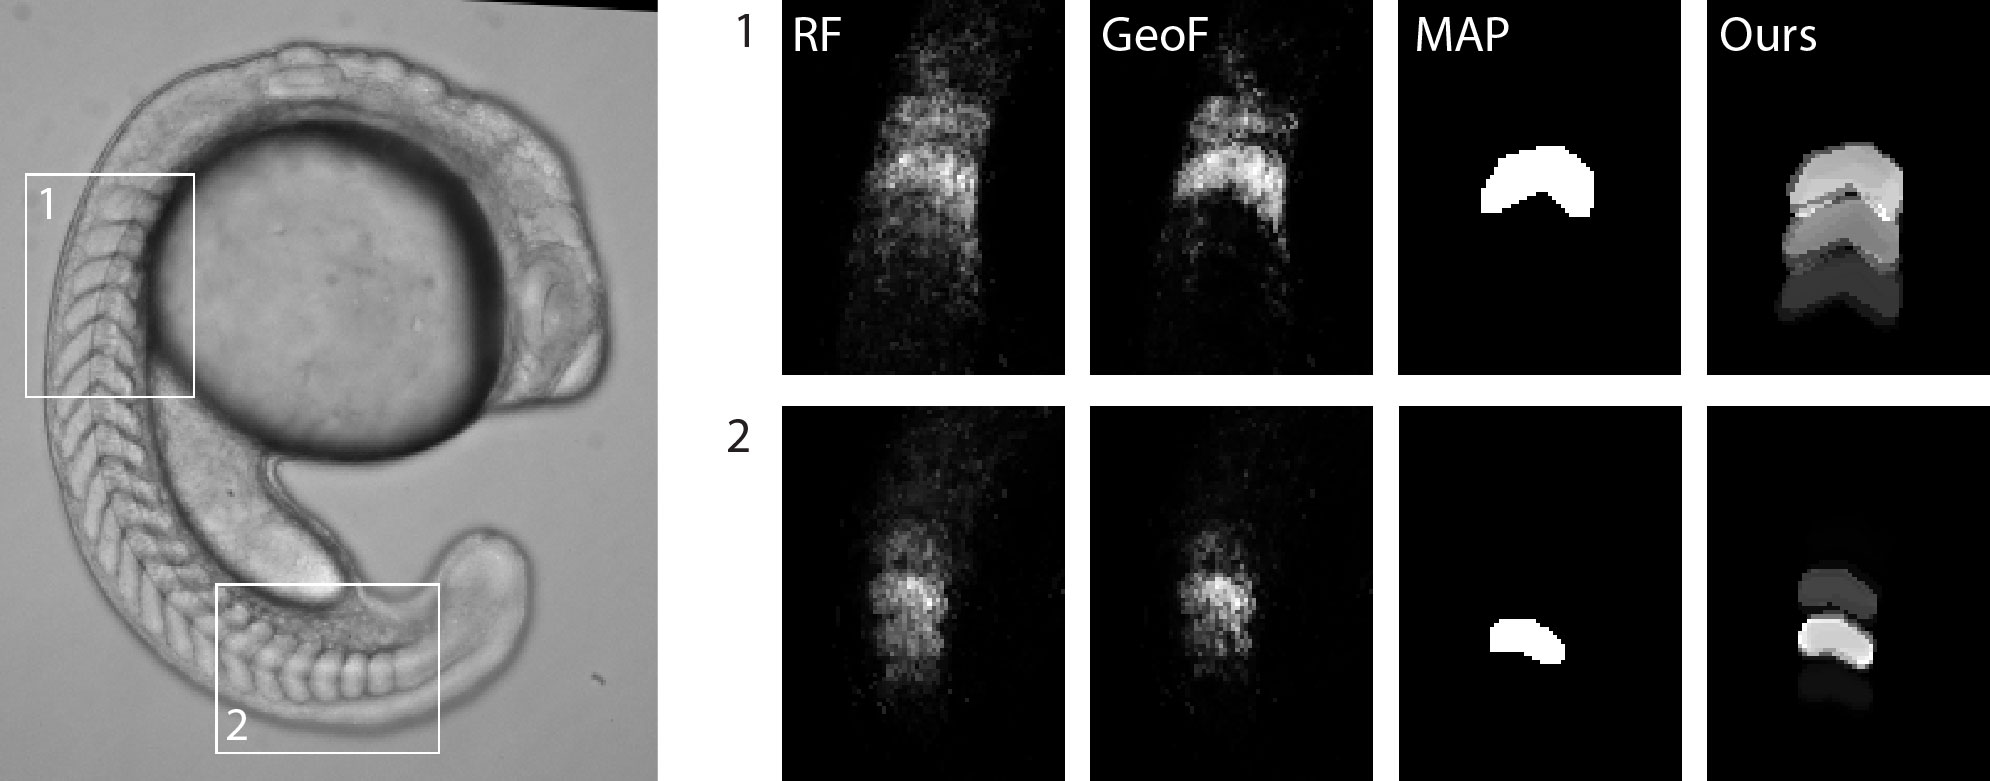
\includegraphics[width=\columnwidth]{smoothing.jpg} %&[trim=0cm 2cm 0cm 1cm,height=0.2\textheight]
\caption{In our evaluation we interleave different types of inference/smoothing into our cascaded random forest pipeline for semantic segmentation of somites (i.e.\ vertebrae) in zebra-fish embryos. 
%
The Figure shows examples of the types of inference/smoothing we evaluate. 
Left: Exemplary zebra-fish embryo. Boxes (1,2): Exemplary somites. Right: Close-ups on probability maps of the respective class labels. Note that close-ups on (2) are rotated by 90 degrees. 
%
Four versions of smoothing/inference: (RF) random forest probability map; (GeoF) smoothed by geodesic smoothing\cite{GeoF2013}; (MAP) "`smoothed"' by MAP inference in our constellation model, yielding a binary "`probability map"'; 
%
(MM) "`smoothed"' by our proposed approach, i.e.\ probabilistic inference in our constellation model.  }
\label{fig:smoothing}
\end{center}
\end{figure}
%


\paragraph{Ours. }

XX remove or expand.  Our approach is inspired by the success of stacked classifiers, such as autocontext, and the observation that feature smoothing is a promising approach for introducing prior information into the learning process.

We begin by training a random forest of 16 trees, each with maximum depth 12, on features stemming from a standard filter bank.  These features are precomputed using the Weka Trainable Segmentation Plug-In (FIJI).  Additionally, we employ the use of contextual features which have been shown to perform very well in anatomical labeling tasks (XX ref Criminisi).  Contextual features are generated by evaluating the filter bank response at a random offset to the current pixel, and either thresholding on this value directly, or taking the difference between this value at the current pixel.  We find that the use of contextual features is essential for disambiguating between segments with near identical appearance and giving a good initialization of the constellation model.  These parameters are used during the comparison of all the following methods.

During training, we use a different subset of the data at each level of the cascade, to avoid overfitting the small data set.  Additionally, we generate two additional random rotations (+/- 10 degrees) for each training instance.  The remaining data at each level is then used to build a constellation model for the backbone, and an active appearance model for every individual segment.  To initialize the AAMs for fitting, we find the mode of the RF output for each class using mean shift, and then fit the rigid constellation model to this.  We additionally recenter each AAM on the mode of RF output for its corresponding class.  From these two sets of initializations, we generate many more by sampling locally along the axis of the constellation model, and then run gradient descent to fit each AAM instance to the input image.  Fitting is done over 6 parameters, one shape parameter, one appearance parameter, and an additional four parameters for the similarity transformation.

Each AAM fit yields a hypothetical segmentation of the corresponding class; however, there is not yet any global consistency imposed.  To introduce this feature, we do probabilistic inference over the chain using Belief Propagation.  The resulting marginals are then used to scale the mask of the corresponding fit, and finally a posterior probability distribution is calculated for every pixel by renormalizing the weighted fit masks over all classes (XX see equation 2?).  See \ref{fig:smoothing}, MM.


\paragraph{Auto Context. }

The canonical example of stacked classifiers is Auto-context, where the RF output is sampled over a regular grid of offsets, and these features are used in the next level of a cascade.  We evaluate the performace of Auto-context by directly using the RF output as input to the next layer, without model fitting.  See \ref{fig:smoothing}, RF, for examples of this.

\paragraph{GeoF. }
The simplest way to generate a smoothed RF Output is to re-use the Geodesic smoothing idea from Criminisi.  Let:

\[ Q(x; M, \nabla I) = \min_{x'} (\delta (x,x') + \nu M) \]

and $\nu$ is some free parameter.  Note, x and x' are two points in the image. $M(x') = 1 - p(c|v(x'))$, where v(x') is the feature vector at pixel x'.  Then the smoothed RF output is calculated as:

\[ g(c|v(x)) = \frac{1}{Z} p(c|v(x)) e^{\frac{-Q(x;p(c|v(\Omega)),\nabla J)^2}{\sigma ^2}} \]

This accomplishes smoothing in quite an indirect way, as a competition between different possible class labels for a given pixel, mediated by the normalization Z.  See \ref{fig:smoothing}, GeoF, for examples of this.

\paragraph{MAP Inference. }

Finally, we consider another model-based method of using.  This approach is exteremely similar to ours; however at every level, the MAP solution of the constellation model is used as features to the next layer.  This returns hard 0-1 decisions about the class of every pixel, see \ref{fig:smoothing}, MAP.

\paragraph{Quantitative Results}

Autocontext is the simplest approach that we consider, and it returns a final Dice score of 0.60 (sd=0.20) after three levels (\ref{tab:results}).  Interestingly, 


talk about cascade boxplots and table (below)

\begin{figure}[t]
\begin{center}
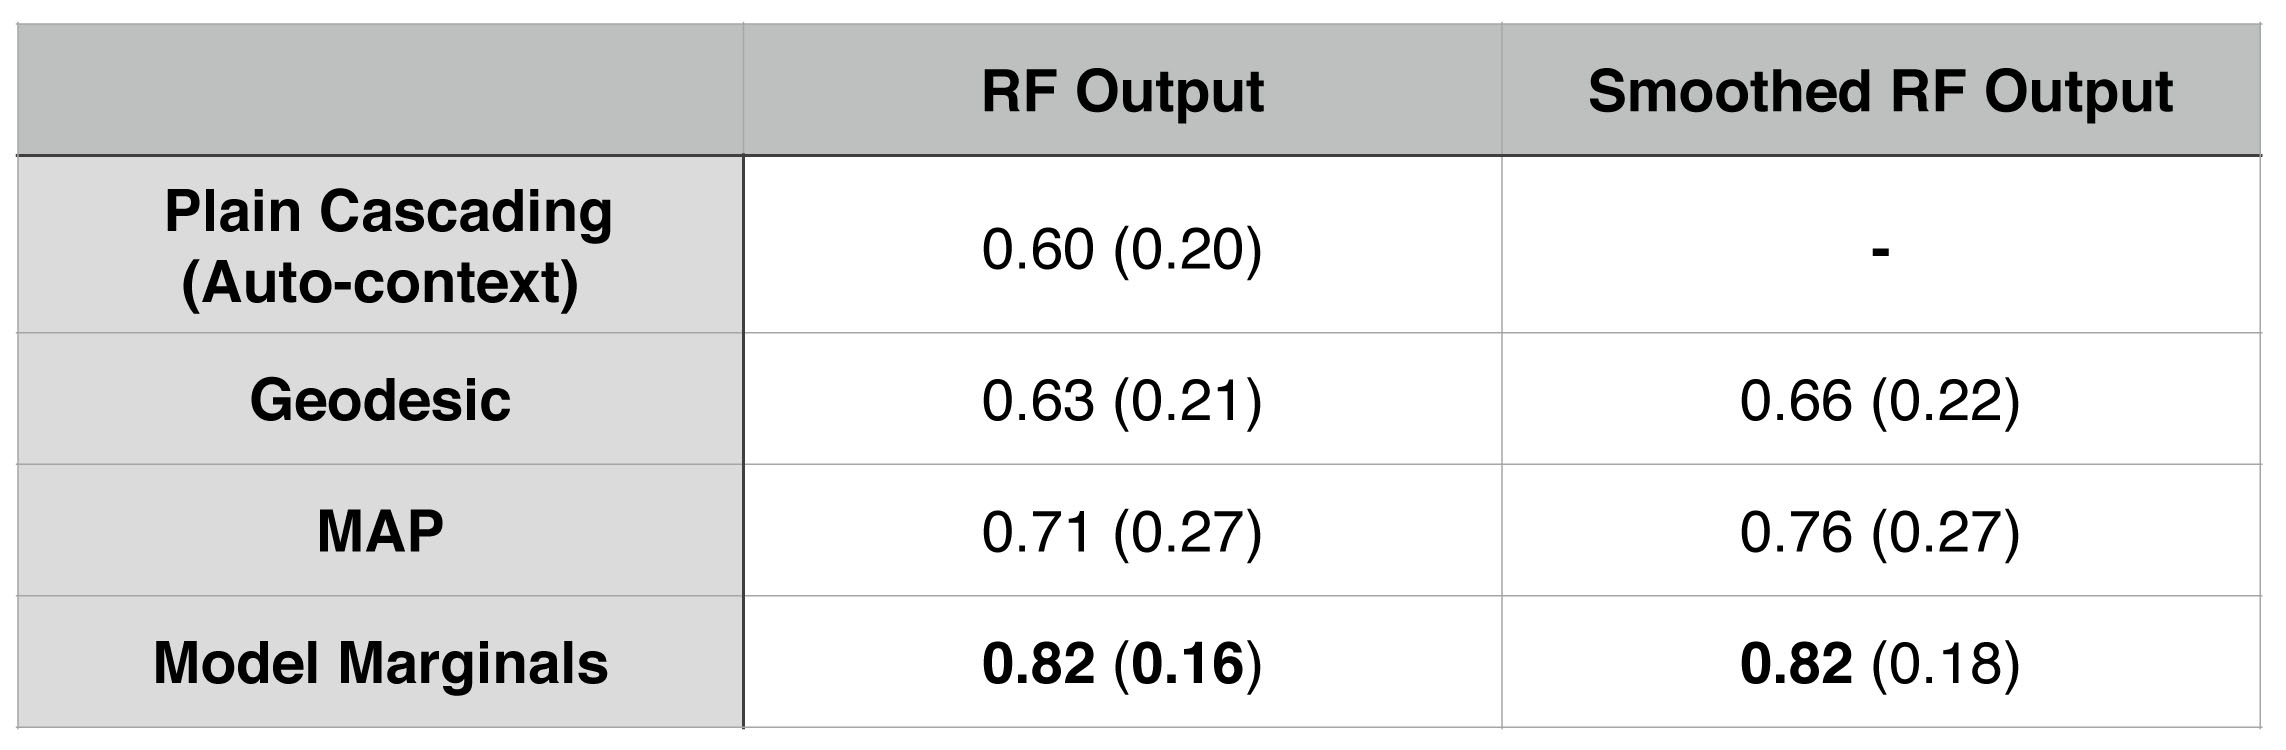
\includegraphics[width=\columnwidth]{TableDiceScores_2columns_noGeoF2.jpg} %&[trim=0cm 2cm 0cm 1cm,height=0.2\textheight]
\caption{Evaluation on 32 datasets. Dice Scores on all 21 Somites: Mean and standard deviation (in brackets).}
\label{tab:results}
\end{center}
\end{figure}

\begin{figure}[tb]
\centering
\small
\begin{center}
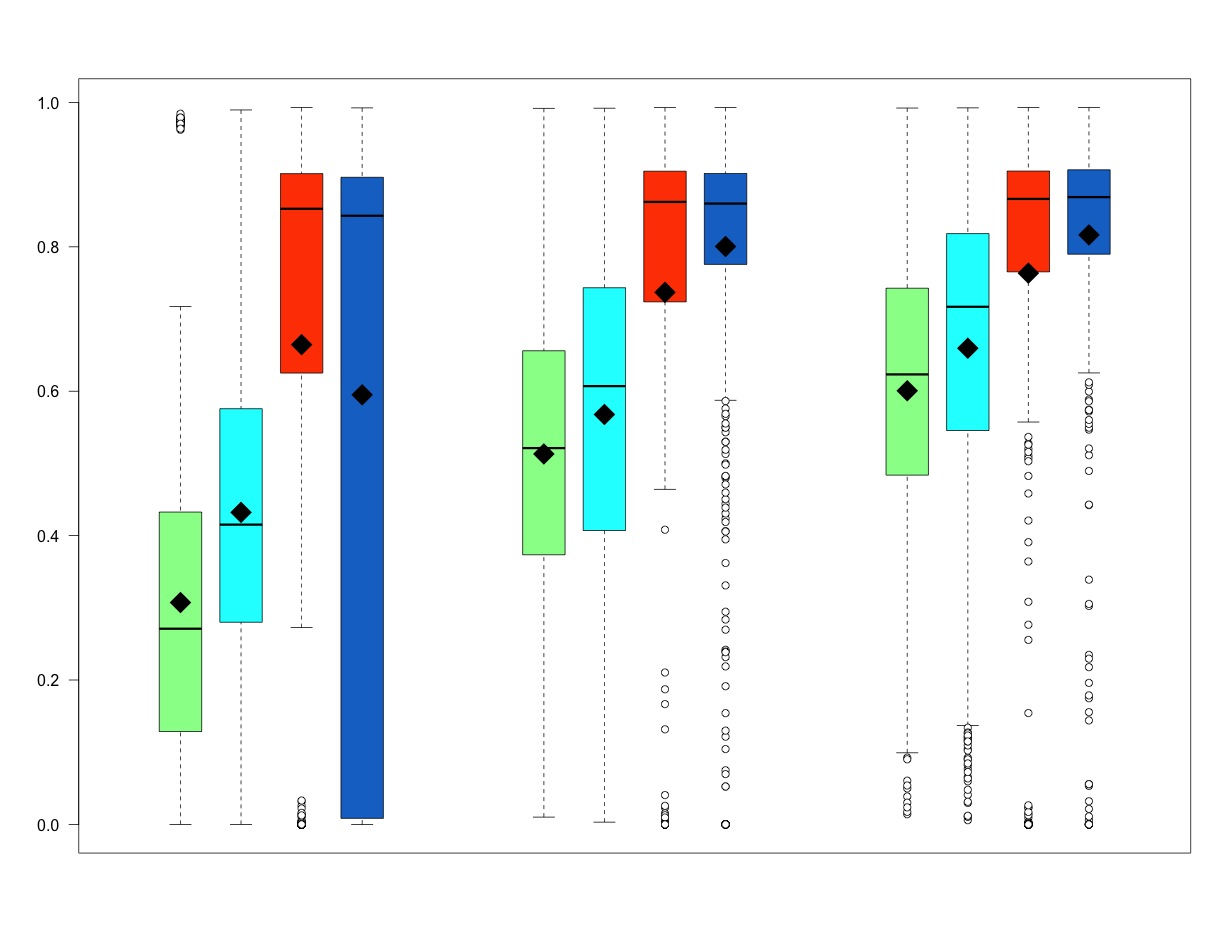
\includegraphics[width=\columnwidth]{Cascade.jpeg} %&[trim=0cm 2cm 0cm 1cm,height=0.2\textheight]
\end{center}
\label{fig:boxplots}
% \vspace{-2mm}
\caption{3 level cascade. Segmentation accuracy of 4 methods after each level: RF output (green), GeoF (cyan), MAP (red), Ours (blue). For every method at every level, Dice scores of 21 somites in 32 images, i.e.\ 672 scores, are visualized as a \emph{box plot}~\cite{chambers1983graphical}. A colored box spans from lower to upper quartile, i.e.\ the inter-quartile range. I.e.\ 50\% of the data points lie within the box. The horizontal bar within the box depicts the median. The black diamond depicts the mean. Whiskers depict the outlier-free data range. Circles depict outliers. Outliers are defined as data points beyond median $\pm$ 2 inter-quartile ranges. }
\end{figure}





\section{Discussion}
Ours is the best :)

\paragraph{Cascading Helps!}
... performance goes up over levels. Boxplots!

... "`traditional"' MAP after one level sucks. 

\paragraph{Smoothing Helps! Model-based Smoothing Helps Best!}
... Auto Context $<$ GeoF $<$ Model Based. Reason: More Specific Prior knowledge...

\paragraph{Uncertainty Helps!}
... Probabilistic inference considerably outperforms MAP inference (6\% better). Reason: With Prob.\ inference, cases can be rescued if not caught after first level (i.e.\ "`at first site"'). Show some rescue cases. 

We also tried MAP after third level. Once all cases are rescued, MAP is fine (performs equally -- state numbers). BUT NOT EARLIER!

Dave, in the rescue figure, please call the bottom row "`Ours"', and maybe re-arrange rows as columns so that the figure fits into one column without being too small. 
\begin{figure}[t]
\begin{center}
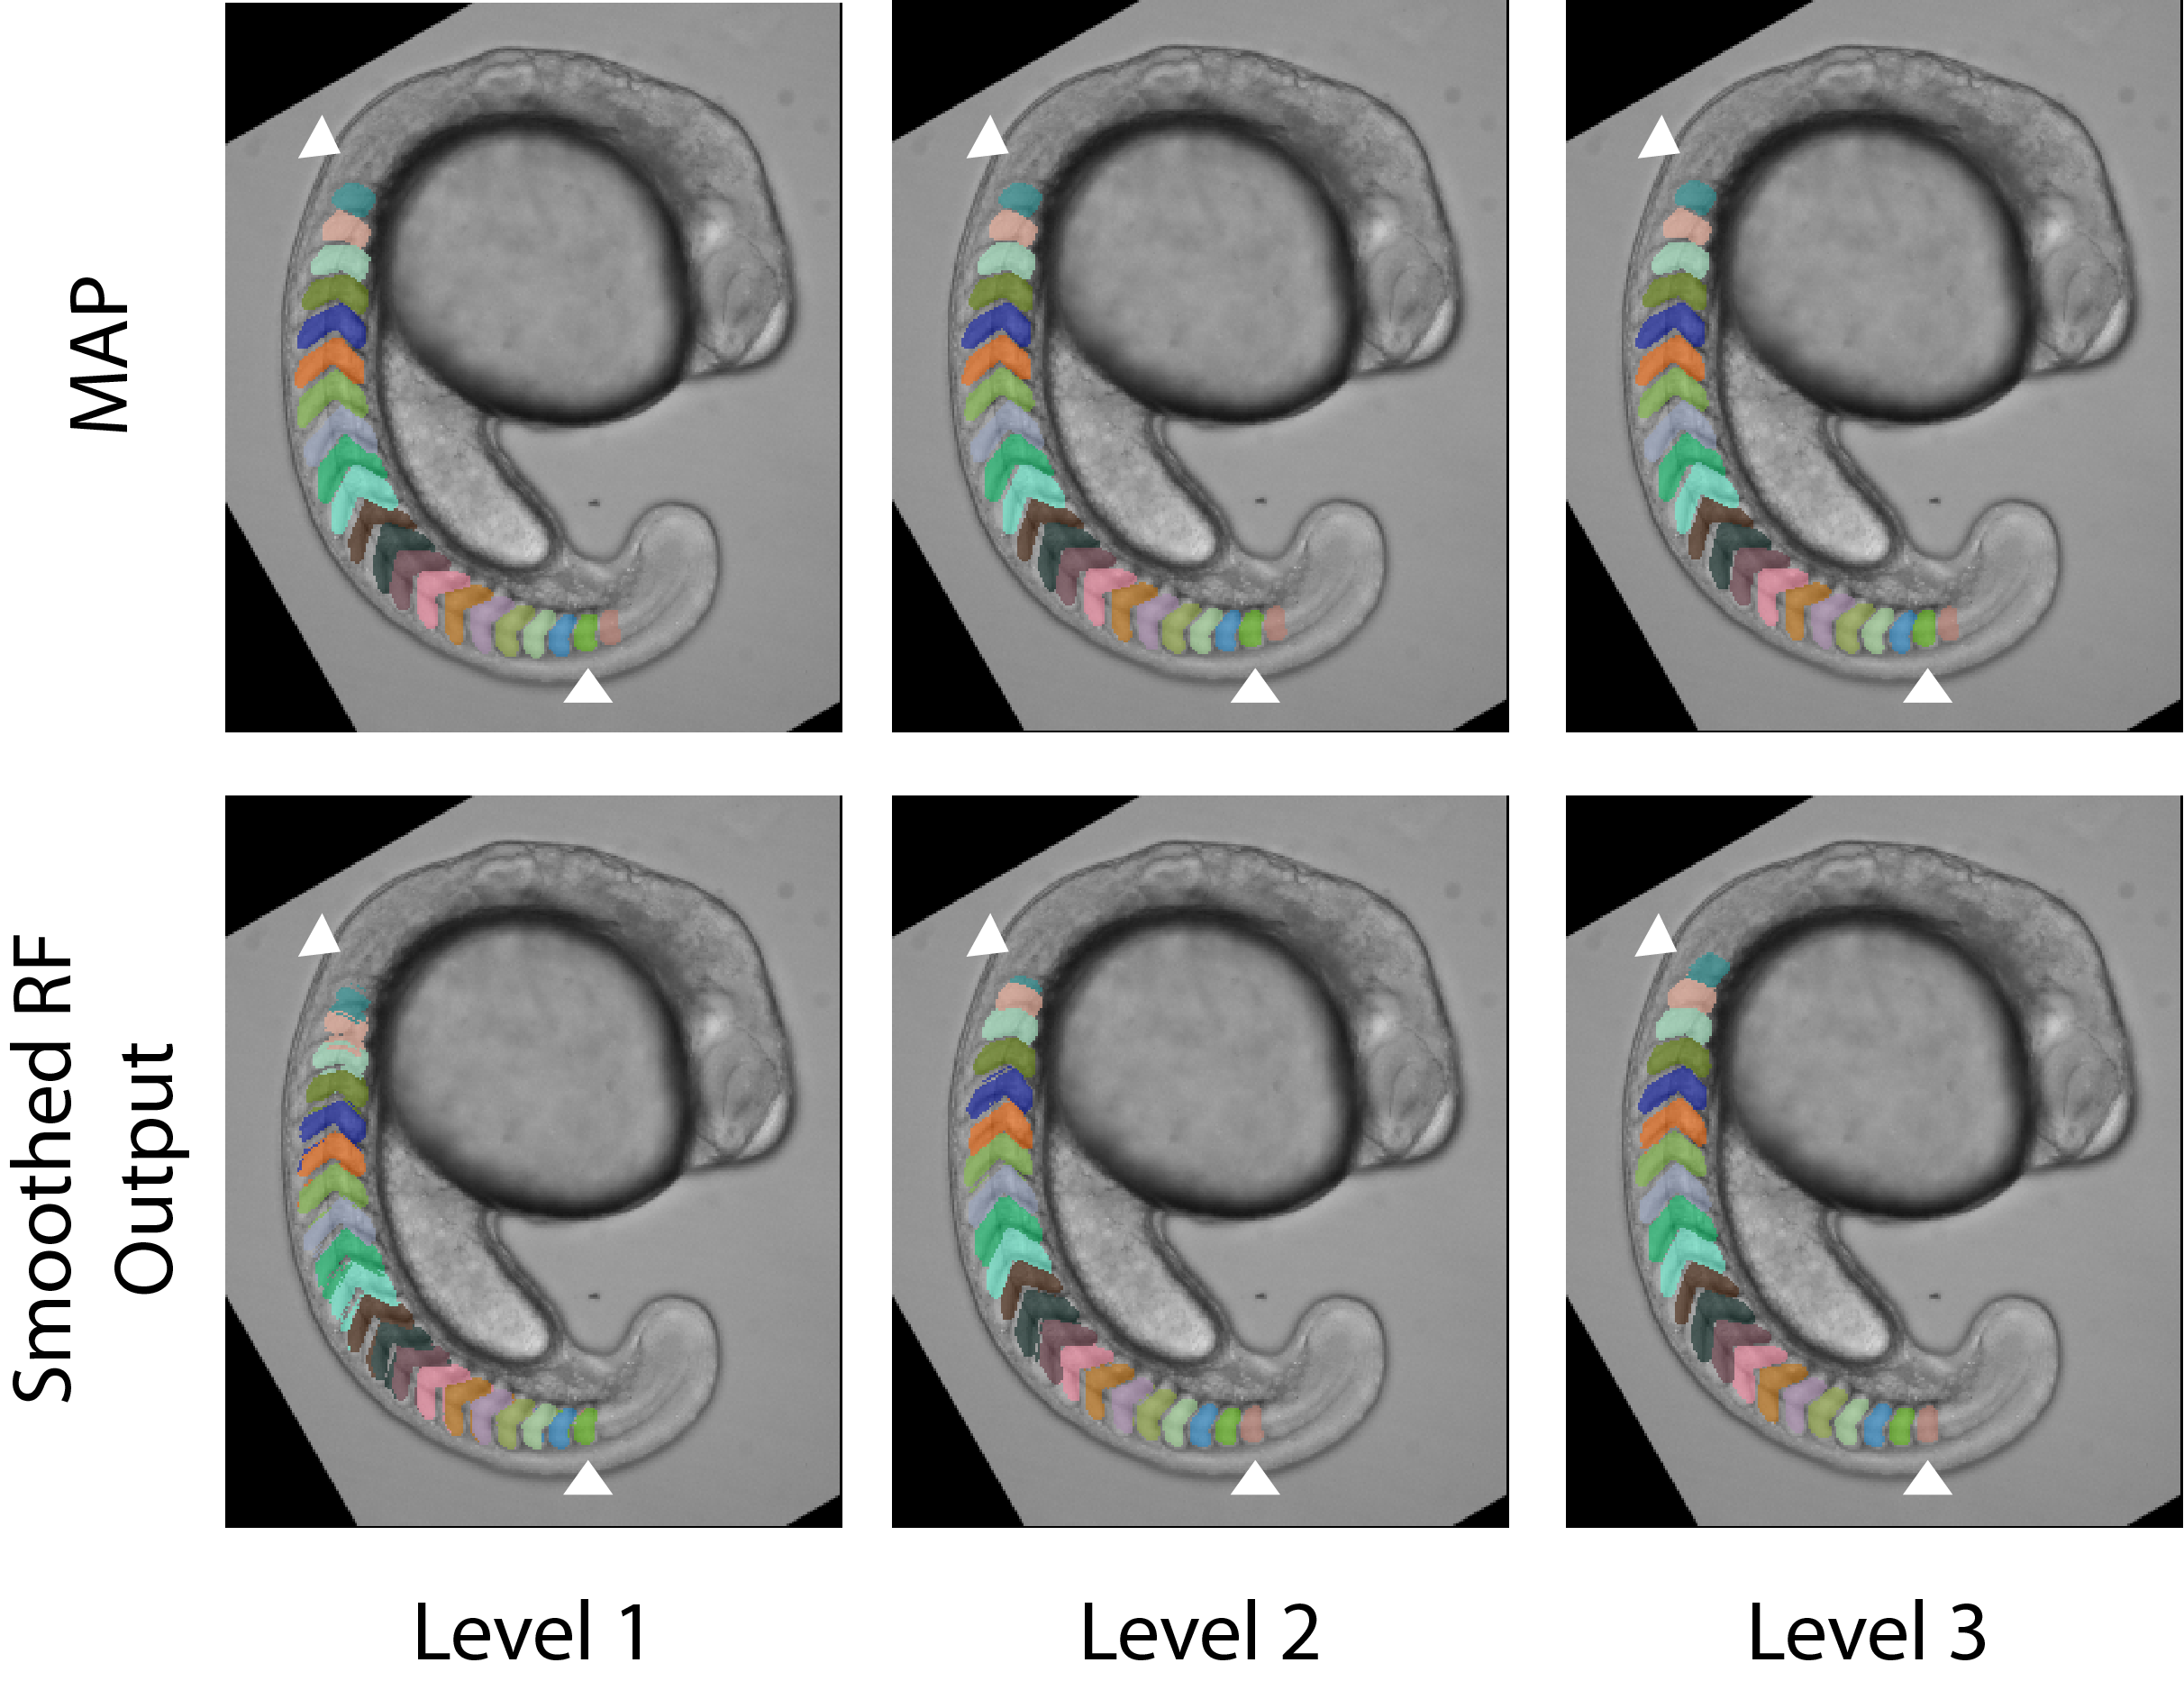
\includegraphics[width=\columnwidth]{rescue.png} %&[trim=0cm 2cm 0cm 1cm,height=0.2\textheight]
\caption{Rescue Case. Arrows point to ground truth start end end of spine. }
\label{fig:rescue}
\end{center}
\end{figure}



{\small
\bibliographystyle{ieee}
\bibliography{somites2014}
}

\end{document}
